\documentclass{article}
\usepackage[margin=1.5in]{geometry} % just to fix margins
\usepackage{setspace}
\usepackage{graphicx} % for graphics (figures)
\usepackage{float} % to keep figures on the same page as its written
\usepackage{titlesec}
\usepackage[parfill]{parskip} % new line between paragraph, no indentation
\usepackage{color} % for color text
\usepackage[font={small,it}]{caption} % side-by-side figures; changing font
\usepackage{times}
% \usepackage{mathptmx}
% \usepackage[scaled=.90]{helvet}
% \usepackage{courier}
%\usepackage{microtype}
\usepackage{subcaption} % for side-by-side figures
\usepackage{url} % for showing raw links
%\usepackage{supertech}
\usepackage{supertech-sig}
\linespread{0.9}

\newcommand{\wchnote}[1]{\cnote{green}{WCH: #1}}

\begin{document}
\newcommand{\figuretitle}[1]{\textbf{#1}\\\vspace{2mm}}

\begin{center}
{\huge Quantifying the Capacity Limitations of Hardware Transactional
Memory}
\end{center}

% \begin{center}
% \begin{minipage}{.9\textwidth}
% \begin{center}
% {\large \textbf{Abstract}}
% \end{center}
\begin{abstract}
Hardware transactional memory (HTM) is a promising solution to the synchronization
problem in multicore software due to its simple semantics and superior performance
relative to coarse-grained locks.
Hardware transactions offer a performance advantage
over software implementations by harnessing the power
of existing cache coherence mechanisms which are already
fast, automatic, and parallel. 
The source of superior performance, however, is also the root of their
weakness: existing implementations of hardware transactions 
will abort when the working set exceeds the
capacity of the underlying hardware.
Before we can incorporate this nascent technology into high-performing
concurrent data structures, 
it is necessary to first investigate the physical capacity
constraints of hardware transactions to inform the design
of such data structures.
We were able to divine details of the HTM implementation
of Intel's Haswell and IBM's Power8 architectures from 
our investigation of the capacity constraints and these 
characterizations provide much needed understanding of the
systems for which practitioners design algorithms and 
data structures.
\end{abstract}
% \end{minipage}
% \end{center}
 

\section{Introduction}
% Random notes:
% \begin{itemize}
% \item Use \defn{defn} blocks to define terms, such as 
% \defn{hardware transactional memory}.  However, \defn{defn} 
% blocks should always have an accompanying definition.  Their
% use is a good mnemonic for remembering that one should define
% important terms.
% \item In text, \textit{italics} or \emph{emphasis} blocks
% are used to draw attention to an otherwise well-defined term
% or phrase.  
% \end{itemize}




As Moore's law plateaus~\cite{Vardi14} the transition
to multicore microprocessors is in full swing. High-performing concurrent
programs require the effective utilization of these multicore chips, but 
synchronization overhead and complexity has been a
major roadblock to building fast concurrent programs.
Transactional memory~\cite{HerlihyMo93} was originally
proposed as a programming abstraction that could achieve
high performance while maintaining the simplicity of 
coarse-grained locks~\cite{YooHuLa13}.
Recently, Intel~\cite{Reinders12,IntelISAX12} and
IBM~\cite{CainMiFr13,Merritt11,IBMPower8Overview14} have both
introduced mainstream multicores supporting restricted \defn{hardware
transactional memory} (HTM) and a new ingredient in the solution 
to the synchronization problem is on the horizon. The Intel and IBM
systems are both \emph{restricted} in that they are 
a \emph{best effort} hardware transactional memory
system~\cite{Roman12,IntelISAX12,CainMiFr13,IBMPower8Optimization14}.
This means that there is no guarantee that an attempted 
transaction will complete successfully, even in the absence 
of memory contention from other cores, due to hardware restrictions
arising from the imperfect implementation.  
Hardware transactions are faster than traditional
coarse-grained locks and software
transactions~\cite{YooHuLa13}~\cite{CascavalBlMi08}, 
yet they have similar
performance to well-engineered software using fine-grained 
locks and atomic instructions (e.g.
\proc{compare-and-swap}~\cite{Herlihy91})~\cite{YooHuLa13}. 
However, \emph{restricted} HTM introduces a wrinkle into 
this otherwise panacean technology: sometimes transactions
will fail even when executed serially due to limitations
of the underlying hardware implementation.  The conditions
under which such a failure may occur dramatically impacts
whether the complexity of designing a software 
system using restricted HTM
is justified by the expected performance.  Characterizing
these conditions is the goal of this paper. 

\begin{figure}[h]%[ht!]
\centering
\begin{minipage}[b]{.45\linewidth}
\centering
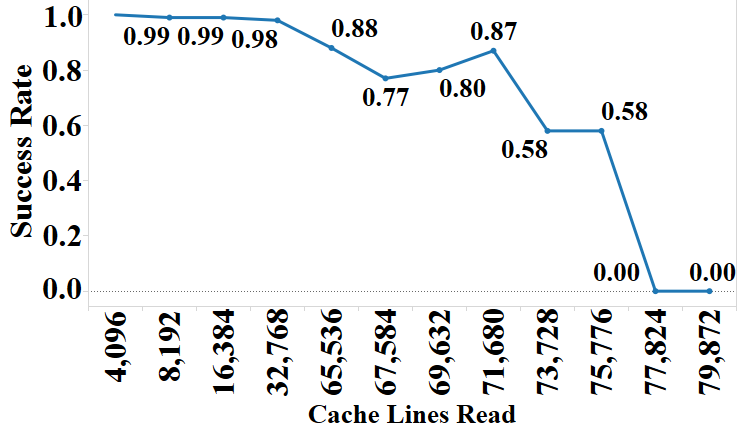
\includegraphics[width=\linewidth]{images/wttm_capacity_read_intel}
\caption{Lines Read vs Success Rate.}
\label{fig:wttm_capacity_read_intel}
\end{minipage}%
\quad
\begin{minipage}[b]{.45\linewidth}
\centering
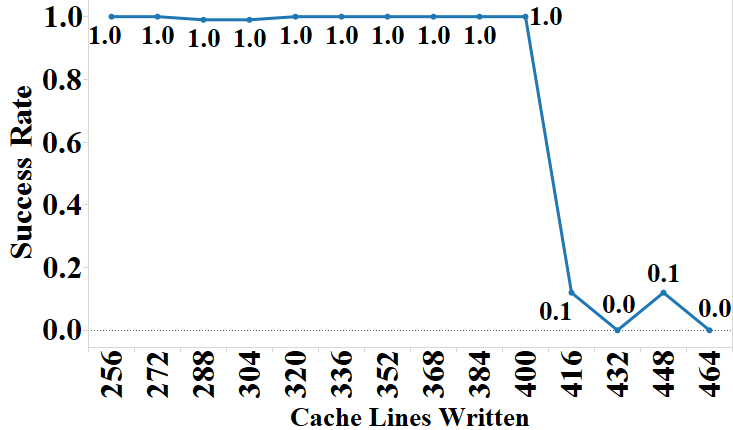
\includegraphics[width=\linewidth]{images/wttm_capacity_write_intel}
\caption{Lines Written vs Success Rate.}
\label{fig:wttm_capacity_write_intel}
\end{minipage}
\end{figure}

Transactions require the logical 
maintenance of \defn{read sets}, the set
of memory locations that are read within a 
transaction, and \defn{write sets}, the set
of memory locations that are written within 
a transaction~\cite{HerlihyMo93}. When transactions execute, 
local reads and writes to memory 
are tracked and recorded in
corresponding read and write sets. Upon 
completion of a transaction, the memory state is validated for 
consistency before the transaction
\defn{commits}, meaning that the modifications to 
memory are visible to other threads.


Transactions may \defn{abort} due to a conflict with
another concurrently executing transaction when an
inconsistent memory state is detected, 
such as when one or many memory locations
in one thread's write set intersects one or 
many memory locations in another
thread's read set or write set.  We call this a
\defn{conflict abort}.  In addition to \defn{conflict aborts},
hardware transactions specifically suffer 
from \textit{capacity aborts} when the underlying hardware
lacks sufficient resources to maintain the
read or write set.

\paragraph{Experimental Setup}
In this paper we summarize results of experiments 
that determine how the
read and write sets are maintained in hardware for recent 
Intel x86 and IBM PowerPC architectures. In particular,
the Intel machine contains a Haswell i7-4770 processor with 4
cores running at 3.4GHz, 8 hardware threads, 64B cache lines, an 8MB
16-way shared L3 cache, 256KB per-core 8-way L2 caches, 
and 32KB per-core 8-way L1 caches.
We also tested an IBM Power8 processor with 10 cores running at 3.4GHz,
80 hardware threads, 128B cache lines, an 80MB 8-way
shared L3 cache, and 64KB per-core 8-way L1 caches.
All experiments are written in C and compiled with GCC, 
optimization level
\texttt{-O0}.\footnote{We compiled with \texttt{-O0} because
we found that higher optimization levels sometimes 
caused spurious transaction
aborts, thus confounding our results.} Our experiments use the GCC
hardware transactional memory intrinsics interface.\footnote{The x86
intrinsics are \texttt{\_xbegin} and \texttt{\_xend}; 
the PowerPC intrinsics are
\texttt{\_\_builtin\_tbegin} and \texttt{\_\_builtin\_tend}.}

The focus of our experiments is to explore scenarios where these
capacity aborts are inevitable so that we know 
when hardware transactions are
not a feasible synchronization solution at all, 
even in the case of no contention. For example, 
\figreftwo{wttm_capacity_read_intel}{wttm_capacity_write_intel}
illustrate the maximum read and write capacity, respectively,
of a hardware transaction on an Intel processor.  In \secref{capacity}
we will explore other types of constraints imposed on
HTM operation by the Intel and IBM implementations.
This characterization should inform
software development attempting to use the newly available HTM support 
and hybrid hardware / software transactional memory
systems~\cite{DamronFeLe06,MatveevSh13}.


\section{Capacity Constraints}
There are physical limitations to the size of hardware transactions that are
governed by how they are implemented in hardware. These capacity constraints
determine when a transaction will inevitably abort, even in the case of zero
contention. It is thus critical to shed light on the hardware implementation of
transactions in order to know when they are not a feasible synchronization
solution at all.

Hardware transactional memory leverages existing caching protocols to maintain
read sets and write sets. As such, we devised an array access experiment to
measure the maximum cache line capacity of sequential read-only and write-only
hardware transactions. We also experimented with strided memory access patterns
to see how different stride amounts affect maximum possible transaction sizes.
With knowledge of the maximum sequential access capacity and also the maximum
strided access capacity, we can draw conclusions about where in the caching
architecture the read sets and write sets are implemented. We report these
results for both the Intel and IBM machines.

\subsection*{Intel}

Figure~\ref{fig:wttm_capacity_read_intel} shows the result of a sequential
read-only access experiment. The data points in the graphs represent the success
probability of the transaction with respect to the number of cache lines read.
The results indicate that a single transaction can reliably read 
around 75000 cache lines and still commit..

Figure~\ref{fig:wttm_stride_read_intel} shows the result of a strided read-only
access experiment. The stride amount is the number of cache lines stepped over
per access. Each data point in the graph represents the maximum number of cache
lines that can be reliably read with respect to the stride amount. For example,
the third data point in the graph indicates that when the stride amount is
$2^2=4$ cache lines stepped over per access, the transaction can reliably read
$2^{14}=16384$ cache lines and commit. The significance of this graph is that
the number of cache lines that can be read in a single transaction is generally
halved as we double the stride amount, presumably because the access pattern
keeps hitting the same few cache sets while completely skipping over other sets.
It is important to note that the plot plateaus at $2^4=16$ cache lines.

Figure~\ref{fig:wttm_capacity_read_intel} and
Figure~\ref{fig:wttm_stride_read_intel} show experimental results that indicate
that the read set is very closely related to, if not directly stored inside, the
\textit{L3} cache. The \textit{L3} cache of this Intel machine has a maximum
capacity of $2^{17}$ cache lines, which explains why read-only transactions
cannot fit much more than $2^{16}=65536$ cache lines because it is impossible
for the whole read set to fit perfectly into the \textit{L3}. The minimum of 16
cache lines readable when the stride amounts are large enough to consecutively
hit the same cache set further supports the notion that the read set is
maintained through the \textit{L3} because this value exactly coincides with the
set associativity of the \textit{L3}, which is 16 cache lines.

Figure~\ref{fig:wttm_capacity_write_intel} illustrates the result of an
identical array access experiment, except now the transactions are write-only
instead of read-only. A single write-only transaction can reliably commit about
400 cache lines.

Figure~\ref{fig:wttm_stride_write_intel} illustrates that the number of cache
lines that can be written in a single transaction is also generally halved as we
double the stride amount, but even as we increase the stride amount
significantly, the number of cache lines that a transaction can reliably write
to does not fall below 8.

The evidence from Figure~\ref{fig:wttm_capacity_write_intel} and
Figure~\ref{fig:wttm_stride_write_intel} suggests that the write set is very
closely related to, if not directly stored inside, the \textit{L1} cache. The
size of the \textit{L1} cache is 512 cache lines, and it makes sense that the
write set can only reach about 400 cache lines because it cannot possibly fit
exactly into the \textit{L1}. The associativity of the \textit{L1} is 8, and
this number coincides with the number of cache lines that can still be written
to for large strided access patterns that hit the same cache set.

\begin{figure}[]%[ht!]
\centering
\figuretitle{Cache Lines Read vs Success Probability}
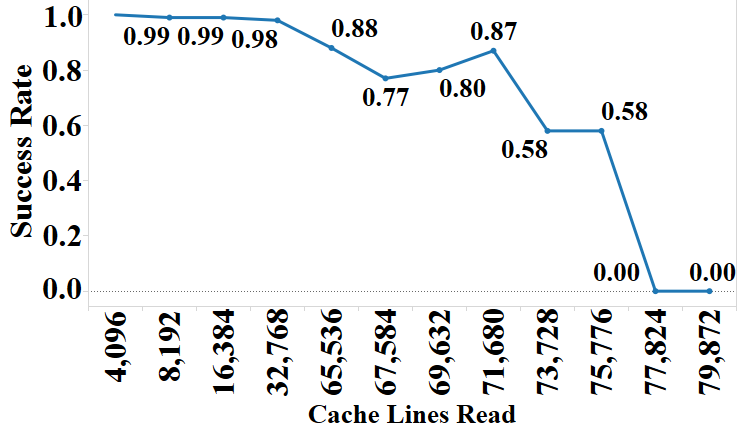
\includegraphics[width=\linewidth]{images/wttm_capacity_read_intel}
\caption{The read set maximum sequential access capacity on the Intel machine is
around 75,000 cache lines}
\label{fig:wttm_capacity_read_intel}
\end{figure}

\begin{figure}[]%[ht!]
\centering
\figuretitle{Stride Amount vs Cache Lines Readable}
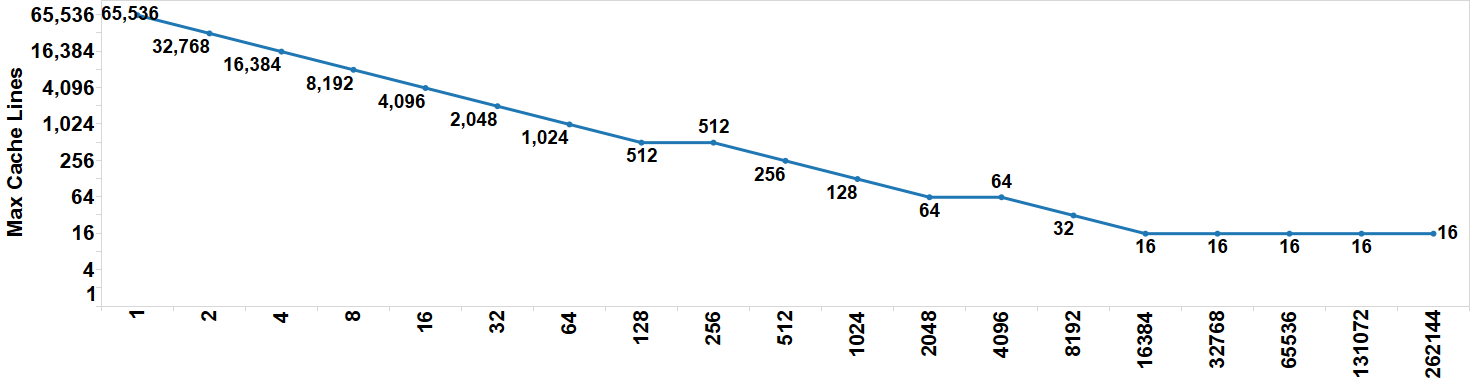
\includegraphics[width=\linewidth]{images/wttm_stride_read_intel}
\caption{Doubling the stride amount halves the size of successful read-only
transactions to a minimum of 16 on the Intel machine}
\label{fig:wttm_stride_read_intel}
\end{figure}

\begin{figure}[]%[ht!]
\centering
\figuretitle{Cache Lines Written vs Success Probability}
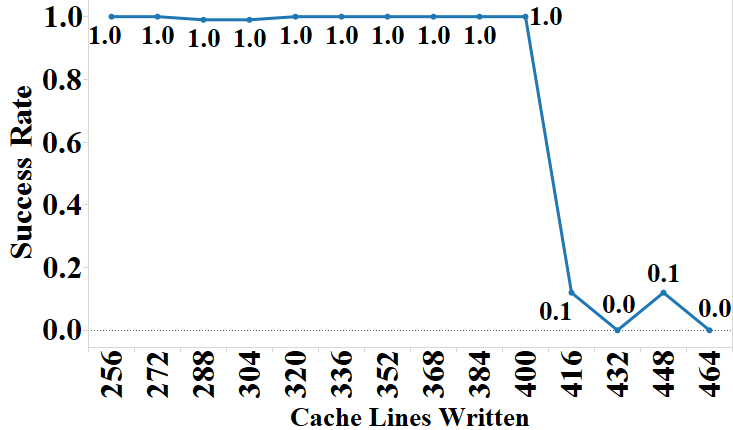
\includegraphics[width=\linewidth]{images/wttm_capacity_write_intel}
\caption{The write set maximum sequential access capacity on the Intel machine is
around 400 cache lines}
\label{fig:wttm_capacity_write_intel}
\end{figure}

\begin{figure}[]%[ht!]
\centering
\figuretitle{Stride Amount vs Cache Lines Writable}
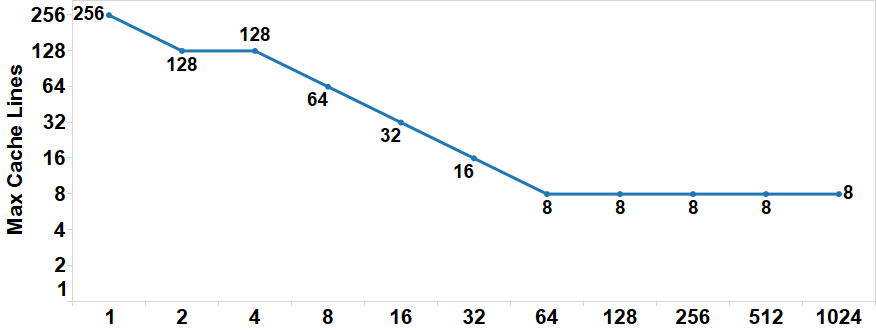
\includegraphics[width=100mm]{images/wttm_stride_write_intel}
\caption{Doubling the stride amount halves the size of successful write-only
transactions to a minimum of 8 on the Intel machine}
\label{fig:wttm_stride_write_intel}
\end{figure}

Judging from the results of our capacity constraint experiments, it is likely
the case that the read set is implemented through the \textit{L3} cache and the
write set is implemented through the \textit{L1} cache on the experimental Intel
machine, and even more generally on other Intel x86 microprocessors that support
hardware transactional memory.

\subsection*{IBM}

Figure~\ref{fig:wttm_capacity_readwrite_ibm} shows that the maximum number of
cache lines that can be read or written in a single hardware transaction on the
IBM machine is very clearly 63 cache lines.

The results of our strided access experiment for both read-only and write-only
transactions appear to be identical in
Figure~\ref{fig:wttm_stride_readwrite_ibm}; the doubling-stride-amount
$\rightarrow$ halving-transaction-size effect is still observed and a minimum of
16 cache lines can be read or written in a single transaction.

The maximum observed hardware transaction size of 63 on this machine is far too
small to be attributed to even the \textit{L1} cache, which holds 512 cache
lines. The identical measurements between the read set and write set found in
Figures~\ref{fig:wttm_capacity_readwrite_ibm}
and~\ref{fig:wttm_stride_readwrite_ibm} suggest that there is little distinction
between the handling of reads and writes in a transaction on the IBM machine.
From these results, we conclude that there are dedicated caches for transactions
on the IBM machine and, more generally, for the PowerPC architecture. The
dedicated caches likely each have 4 cache sets and a set associativity of 16,
for a total of 64 cache lines.

\begin{figure}[]%[ht!]
\centering
\figuretitle{Cache Lines Read/Written vs Success Probability}
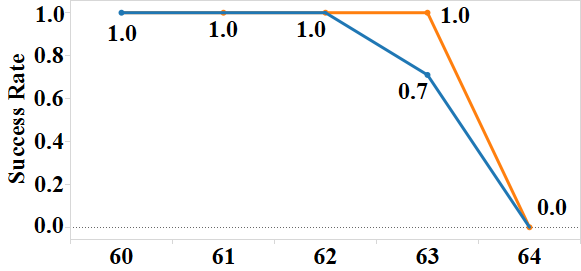
\includegraphics[width=\linewidth]{images/wttm_capacity_readwrite_ibm}
\caption{The read set and write set maximum sequential access capacity on the
IBM machine is 63 cache lines}
\label{fig:wttm_capacity_readwrite_ibm}
\end{figure}

\begin{figure}[]%[ht!]
\centering
\figuretitle{Stride Amount vs Cache Lines Readable/Writeable}
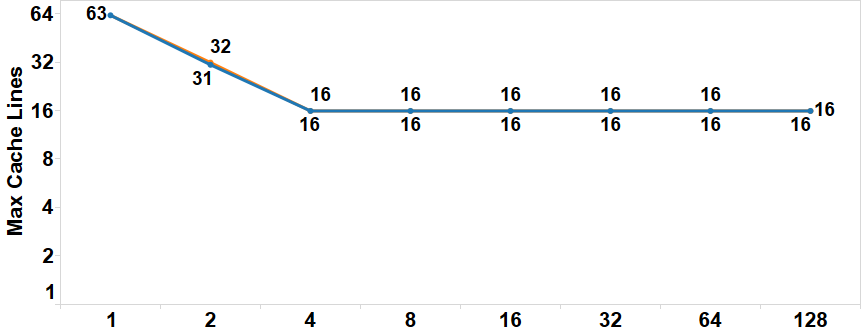
\includegraphics[width=100mm]{images/wttm_stride_readwrite_ibm}
\caption{Doubling the stride amount halves the size of successful read-only and
write-only transactions to a minimum of 16 on the IBM machine}
\label{fig:wttm_stride_readwrite_ibm}
\end{figure}

\begin{figure}[]%[ht!]
\centering
\figuretitle{Num Threads vs Committed Transactions}
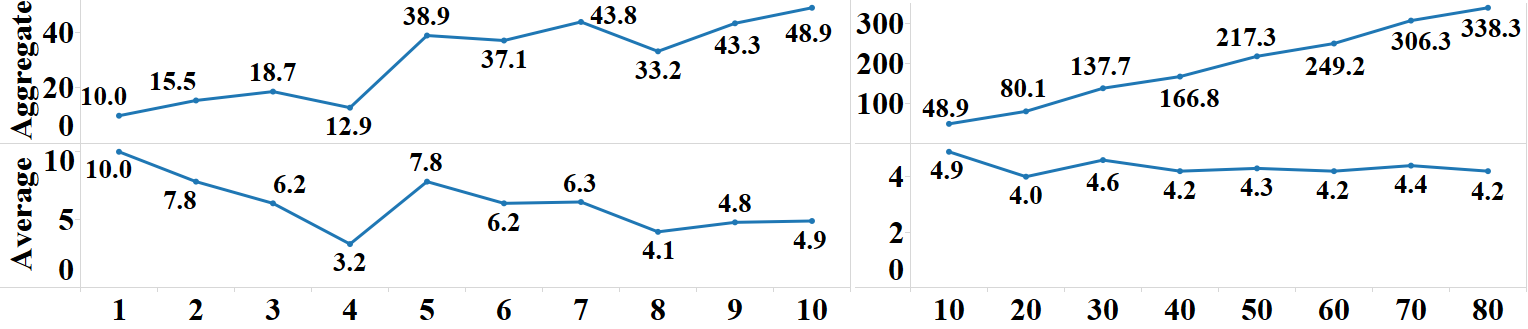
\includegraphics[width=\linewidth]{images/wttm_core_or_thread_ibm}
\caption{Aggregate committed transactions increases with the number of threads
while average committed transactions remains constant, suggesting that there is
a dedicated cache per core on the IBM machine}
\label{fig:wttm_core_or_thread_ibm}
\end{figure}

A natural next question is whether this IBM machine has 10 dedicated caches that
are spread across each core, or if there are 80 dedicated caches that are spread
across each hardware thread. To determine the difference, we experimented and
measured the number of successful write-only transactions that concurrently
running threads were able to complete. Each thread makes 10000 transaction
attempts to write 40 thread-local padded cache lines and then commit. The
transaction size of 40 cache lines is designed to sufficiently fill up the
dedicated caches per transaction to induce capacity aborts in the case of shared
caches.

We see in Figure~\ref{fig:wttm_core_or_thread_ibm} compelling reason to believe that
there are 80 dedicated caches, one for each hardware thread. Each spawned
software thread is pinned to a unique hardware thread in round robin fashion
such that the distribution is even across the 10 cores. If all 8 of the
hardware threads on a single core share a single dedicated cache, we would
expect to see sublinear speedup, perhaps even degraded performance, as we spawn
more running threads and assign them to the same core. Instead, we observe a
linear increase in the aggregate number of successfully committed transactions,
while the average per-thread number of successful transactions is constant.
Although the general 45\% success rate suggests some level of contention between
the running threads, it is most likely not due to per-core sharing of a
dedicated cache.
 


\section{Conclusion}
Hardware transactional memory is an exciting new solution to the synchronization
problem in multicore software. Before we can effectively use this new
technology, we must first understand the physical limits of hardware
transactions that are inherent to the Intel and IBM microprocessors on which
they are implemented. Our capacity constraint benchmarks revealed that the read
sets are implemented through the {L3} and the write sets are implemented through
the {L1} on the Intel machine; on the other hand, there is a
per-hardware-thread, 4-set, 16-way dedicated cache that maintains the read and
write sets on the IBM machine.

Developers using HTM on Intel's Haswell microprocessors have a lot of
flexibility with hardware transaction size, but they should be wary of how the
caching behavior of non-transactional code might affect HTM performance.
Practitioners on IBM's PowerPC microprocessors should be cautious of the tight
restriction on transaction size, but fortunately they only need to reason about
HTM performance within the scope of a single hardware thread.

We anticipate that these findings will move us in the right direction to better
understanding hardware transactional memory, ultimately enabling its
proliferation into future concurrent programs.
 


\bibliographystyle{abbrv}
\small\bibliography{allpapers}

\end{document}



















